% ssb-paper-2018/main.tex

\documentclass[sigconf]{acmart}

\title{Secure Scuttlebutt: An Information-Centric Protocol for
  Subjective and Decentralized Community Applications\\
\tt\small ( \today\ / last commit was \input{.git/refs/heads/master})}

% \title{Replicated append-only logs as as basis for decentralized
% information-centric applications: An analysis of Secure Scuttlebutt}

\author{Dominic Tarr}
\affiliation{ssb:@EMovhfIrFk4NihAKnRNhrf}
\email{RaqIhBv1Wj8pTxJNgvCCY=.ed25519}

\author{Erick Lavoie}
\affiliation{McGill University, Montreal, Canada}
\email{erick.lavoie@mail.mcgill.ca}

\author{Aljoscha Meyer}
\affiliation{TU Berlin, Germany}
\email{???@tu-berlin.de}

\author{Christian Tschudin}
\affiliation{University of Basel, Switzerland}
\email{christian.tschudin@unibas.ch}


\acmConference[XYZ'19]{ACM XYZ conference}{Sep 2019}{Place, Country}
\acmYear{2019}
\copyrightyear{2019}
\setcopyright{rightsretained}

% ----------------------------------------------------------------------
\begin{document}

\begin{abstract}
  Secure Scuttlebutt (SSB) is a novel peer-to-peer information-centric
  event-sharing protocol and architecture for social apps. In this
  paper we describe SSB's features, its operations as well as the
  rationale behind the design. We also provide a comparison with
  traditional information-centric networking protocols and discuss
  SSB's limitations and evolution opportunities.

  At the transport level, SSB is a replication protocol for
  append-only logs.  applications communicate indirectly by writing to
  the local node's log and by reading from the locally available
  replicated logs. From these, each app instance constructs its own
  intepretation of the shared app state (an approach called
  ``subjective reader'').  Scaling is achieved through in-network
  caching of the immutable log updates and by routing the content
  along the social graph.

  SSB's current set of applications include classical social media
  apps (chat, with end-to-end encryption and meta-data privacy), game
  and lifestyle apps (chess, book reviews) as well as technical
  applications like a p2p git, a shared file system, or a social
  backup app for crypto keys using a secret sharing protocol.
\end{abstract}

\maketitle


% ----------------------------------------------------------------------
\section{Introduction}

A simple conceptual architecture for community applications consists
of a global data pool to which every person can contribute and where
every person can tap into the shared data~-- data sharing being the
purpose of such applications. This model still is valid if one adds
access control to the picture, either tied to the data (encryption
giving access to content only to entitled holders of the decryption
keys) or encrypting data in transit (login and TLS). Facebook and
other centrally organized social app service providers fit well under
this global data pool model but have been strongly criticized for
abusing their central provisioning position.  The ``decentralized web
movement''~\cite{decent-2018-aug} is the most visible technical
response to this critique, pointing out implementation alternatives.

One of these alternatives is a project called Secure Scuttlebutt (SSB)
that started in 2012. After several iterations of protocol design and
implementation, SSB has become a stable service for over 10,000 users
offering them rich media community applications with strong
cryptographic protection (end-to-end encryption and metadata privacy)
and running in pure peer-to-peer mode.

\subsection*{Selective Complete Log Replication}

SSB's spin on the above conceptual model is that all participants {\em
  replicate the global data pool}, which enables off-line operations,
avoids redundant data transfers and has become feasible --~at least in
principle~-- because storage nowadays is a cheap resource, just that
the sheer volume of social app data prohibits a full
replication. However, because a participant is mostly interested in
content from its peers, which is a very small number compared to all
participants, only portions of the global data pool need be
replicated. This observation is leveraged in SSB's transport layer
which is tasked to {\em selectively replicate} the global data pool
{\em along the edges of the social graph}, as we will explain in
Section~\ref{sect:XX}.

\begin{figure}[htb]
  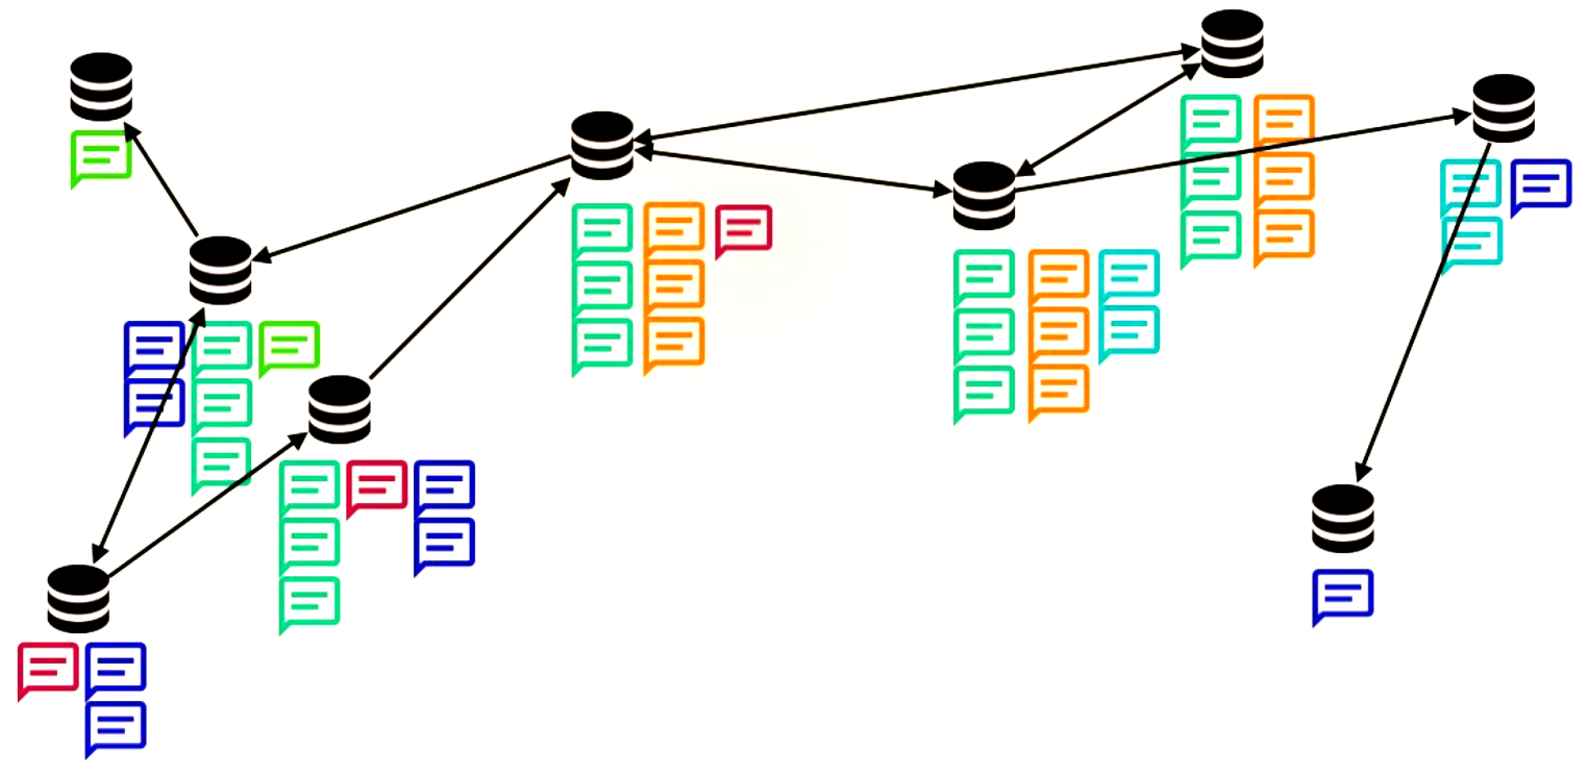
\includegraphics[width=0.9\columnwidth]{figs/staltz-iop.pdf}
  \caption{Staltz' ``Internet of People'' figure, needs to be redrawn
    such that it can be read in B/W, too.}
\end{figure}

A second spin of SSB is that replication is done {\em pro-actively} and
at the granularity of the {\em complete input by a single peer} to the
global data pool. This novel way of implementing the global data pool
model is in stark contrast to current solutions where central server
repositories hosting this pool are accessed by client software in an
on-demand fashion, assuming a storage-less end-device. Today's data
dissemination mode is reactive (client-server protocol to fetch data)
and piece meal (only the instantly needed data items are requested,
possibly multiple times, and bundled with fresh ads, as the client
does not necessarily cache all requested data). In SSB however, the
central objects are the {\em complete} collection of a specific peer's
input to the pool, organized as an append-only log. In
Sections~\ref{sect:XX} and~\ref{sect:XX} we will explain the
advantages of this approach (trust, off-line operations and efficient
real-time notifications), and discuss its drawbacks (index building,
lack of delete operation, storage bloat, re-keying).

\subsection*{Subjective Reader}

Because replication in SSB is selective and is driven by a peer's
social graph, different end devices will have access to different sets
of log replicas, leading to different views of the world which is also
called a ``subjective reader'' approach. SSB's viewpoint is that this
is not a deficit but a desirable property: Each peer is free to
consider data sources of its own choosing instead of having to feed
from a centrally provisioned or otherwise converged view. While it is
possible to implement consensus protocols over SSB, or to designate
central data aggregators from which many peers consume the
consolidated outputs, the SSB network itself deliberately doesn't
offer consensus services nor central content (directories etc). In
Section~\ref{sect:XX} we will show the implication of this
technological choice on the structure of distributed applications that
can only read from and write to local logs.

\subsection*{Novelty}

Putting complete replication of individual append-only logs at the
core of SSB's protocol avoids several hard problems in distributed
systems. {\bf First}, it is a radically decentralized approach
requiring only minimal specification-level coordination among the
participants but no run-time checks or configuration
management. Typically, active/active multi-master replication in
databases, which comes closest to SSB's approach, requires tight
configuration control while in SSB, existing peers can go offline and
new peers can come and go at any time, at the price of weak
consistency guarantees, though. {\bf Second}, although append-only
data structures are well known for their benefits and are at the core
of crypto currencies' consensus finding, SSB uses logs without any
consensus properties. Quite on the contrary, SSB completely sidesteps
consensus but provides the hooks for implementing service abstractions
like tangles for implementing CRDTs on top of SSB i.e., eventual
consistency. {\bf Third}, crafting a cryptographic ID system and
maintaining a social graph that informs routing creates a very narrow
filter: it implements a receiver-driven approach (similar to
e.g. Named Data Network, but at a higher object granularity) where
data only flows where it is needed and without imposing any
fine-grained request/reply protocol. Instead, any dissemination
technology is adequate, including broadcast and push mode, because
network elements can verify data validity (due to the logs' signed
entries) and monotonicity of the updates without additional key and
certificate material, guaranteeing that only conformant traffic is
propagated at any forwarding step. {\bf Fourth}, it makes every peer a
publisher by design. This property goes beyond the decentralized
approach like DAT~\cite{} or IPFS~\cite{} which assume that there
exist replication servers but keep the separation between a data
transport network and a server layer. In SSB, bidirectional
communications is only possible if both parties {\em are}
repositories. {\bf Last but not least}, log replication leads to a
distributed system with inherent high resilience as any communicating
element MUST replicate the others' logs. In traditional distributed
systems, coordinating the data persistence as a basis for resilience
is often an add-on task, or requires at least a special recovery
service.


\subsection*{Scuttlebutt = Information-Centric Gossip}

\ldots\ why this name
\ldots\ it applies to the app-level, and can apply to the network layer, but doesn't have to: any dissemination method works for gossip.
\ldots\ some words about the SSB community, available documentation, past evolution, subjective roadmap \cite{ssb-consortium, tarr:ssb-notes,ssb-on-web,ssb-protocol-guide-2018,staltz-roadmap-2019}

\subsection*{Structure of this paper}

\ldots


% ----------------------------------------------------------------------
\section{SSB Architecture and Protocol}

Introduce and explain figure~\ref{fig:waist} here, the role of SSB as
the protocol stack's waist (like IP is for the Internet).

\begin{figure}[htb]
  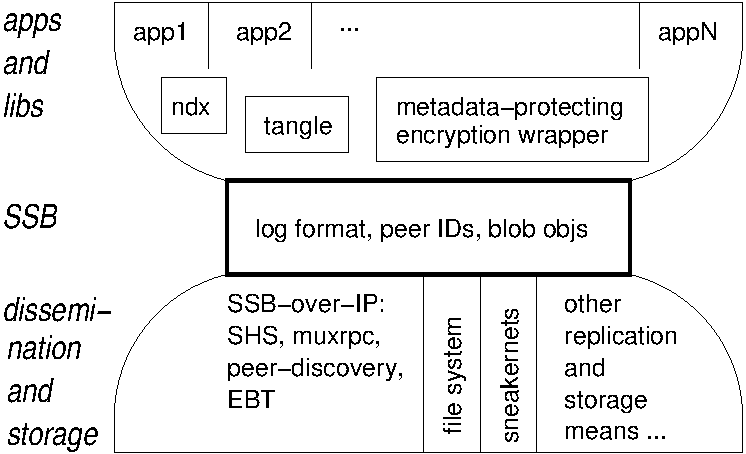
\includegraphics[width=0.9\columnwidth]{figs/ssb-waist.pdf}
  \caption{Secure Scuttlebutt's protocol stack.}
  \label{fig:waist}
\end{figure}

Note: the dissemination/replication layer is able to (and must) read
the logs in order to extract the social graph, responsible for
reachability/forwarding decisions.

\subsection{Identities and their append-only log}

\subsection{Social graph and log replication}

follow, follow-back, block

\subsection{Blobs}

separate content category, own name (independent of logs) and
dissemination protocol

\subsection{Log entry format}

envelope and payload, hashchain entry, JSON

\subsection{E2E encryption and metadata privacy}

\subsection{SSB as an IP overlay, EBT}

\subsection{Secure Handshake (SHS)}

\subsection{SSB Pubs (aka super nodes?)}
\ldots

% ----------------------------------------------------------------------
\section{Distributed Apps and Data Structures over SSB}

{\em Wordsmithing needed:}
The goal of this section: show how SSB's distributed apps can reconstruct
the app's state by parsing the logs, and operate on the app state by
writing to the peer's log. We give more details for SSB's user
directory and also list and quickly characterize other existing
SSB apps. A crucial (performance) aspect is incremental indexing
which we expand on in the subsection about the Kappa approach. More
node-local support in form of libraries and conventions at the level
of log entries is discussed in the subsection on tangles.


\subsection{Example: SSB's user directory}

`{\small\tt about}' is SSB's user database i.e., an application that
associates cryptographic IDs with (typically) human-readable
attributes. A single log entry format has been defined to this end:
{\small\begin{verbatim}
'content': {
  'type'  : 'about',
  'about' : target_id,
  attr_name : attr_value   // multiple times
}
\end{verbatim}}

\noindent
The {\small\tt about} app scans all logs for all entries of type {\small\tt
  `about'} and constructs a database as shown in
Figure~\ref{fig:about}, retaining the most recent attribute assignment
found.  To each target user ID we associate a directory where
key/value pairs are collected on a per author basis (which is extracted
from the log entry's envelope).

Currently the {\small\tt name}, {\small\tt description} and {\small\tt
  image} attributes are understood by most SSB user interfaces and are
used to substitute or decorate the cryptographic ID. If {\small\tt
  target\_id} and {\small\tt author\_id} are identical, the
attributes are self-chosen, and otherwise given.

\begin{figure}[htb]
  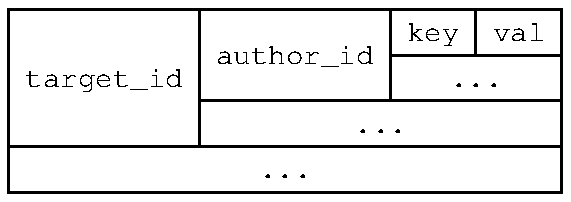
\includegraphics[width=0.6\columnwidth]{figs/about-ds.pdf}
  \caption{SSB's user directory data structure (after extraction from the logs).}
  \label{fig:about}
\end{figure}

\noindent
In terms of CRUD actions, creation happens once a new SSB peer adds
its own {\small\tt about} entry to its log; reading the user database
is performed on the above data structure; updates are expressed by
adding an {\small\tt about} entry --regardless whether it relates to
the peer itself or to another peer-- to one's own log and all peers
updating their extracted database; deleting a user entry is not
possible, at least not directly (one would have to block that user ID
as well as all IDs which wrote an update for that user).

There can never be confusion about the sequence or scope of attribute
assignments because they are orderd by the log (and thus in time) and
kept separate, per author ID. Note also the presence of the
``subjective reader'' property: The content of a peer's user database
is dependent on its position in the social graph. The ``subjective''
mindset is also visible by letting every user assign attributes to
anybody, leaving it to the user interface (and human viewer) to select
which of the self-chosen or given display names and images is most suitable
for a given ID.

\subsection{Profiles of other selected SSB apps}
\label{Section:AppProfiles}

Multiple applications have been written by contributors and are used daily by
the SSB community. We briefly present selected examples because they represent
alternatives to well-known services and they illustrate both opportunities and
challenges of communication through replicated append-only logs.

\textit{Git-ssb}~\cite{git-ssb} is an alternative to GitHub~\cite{github} that
replicates git-based version-controlled code repositories through contributors
logs. It provides an encoding of repositories in SSB logs, a bridge to
interoperate with git repositories, and a web-based viewer to browse
repositories. The object model of Git~\cite{chacon2014pro}, based on immutable
hash-referenced objects organized in a chain of commits, has a similar
structure to SSB's logs, making the mapping natural. Hash objects are blobs and
commits are messages in individual append-only logs.  Other git operations,
such as creating a repository, creating merge commits, creating a branch, or
requesting the merging of an alternative branch (\textit{pull-request}) to a
core maintainer, are all SSB messages. This model provides automatic
distribution of code repositories and their updates through the replication of
SSB logs. Many developers can also update and perform operations on the
\textit{same} repository, as defined by its creation message, independently.
Consensus on the "official" master branch and its latest commit is enforced
through social coordination because the developers of the community know and
trust each other. Nonetheless, in case of concurrent updates to the same branch
in the same repository~\cite{git-ssb-push-conflict}, the git bridge will create
multiple branches when a local git repository is updated. A user can then
resolve the fork by merging the diverging branches and updating the repository.
Referencing both concurrent updates in a later merge commit in effect resolves
the ambiguity through a tangle extension~(Section~\ref{Section:Tangle}).

\textit{Ssb-chess}~\cite{ssb-chess} is a correspondence chess application in
which players can invite one another to play, alternatively share their next
move until the game ends, and external observers can comment on the game. The
core data structure that represent a game is a linked list with nodes
representing chess moves alternating between the two participants' logs. The
detection of invalid moves is performed by the user interface using a
validation library, because participants are trusted to only publish valid
moves on their feed. This latter assumption was made because games are played
between friends in a non-competitive setting. In effect, the validity of the
latest move is implicitly confirmed by the next player choosing to follow with
another move because if they were to disagree on the validity, the conflict can
be handled outside the game and the game can be abandoned. Moreover, a chess
application is easy to encode in append-only logs because the rules of chess
preclude concurrency, i.e. at any time there is always only one of the two
participants that is permitted to modify the state of the chess board by making
a move. The game state also cannot be corrupted by external parties because
only the participants, explicitly mentioned in the original invitation, are
allowed to modify the state of the game. Any non-participant extending the game
with their own move is simply ignored.

\textit{Gatherings}~\cite{patch-gatherings} are alternatives to
Meetup~\cite{meetup.com} that enables participants to signal their intention to
attend or not attend to physical events. Gatherings can be public, in which
case anyone that replicates a log will see them, or private, in which case only
explicitly-invited people will be notified of the event and may signal their
intention. A gathering is defined by its creation message but otherwise has no
fixed properties. Anyone that has a reference to the creation message may
change its properties, such as location, start and end dates, description, and
image, by publishing an update message. The value of those properties are the
most recent set by anyone. Initially, recency was determined by the time of
creation, as reported by the user's client implementation (\textit{self-stated
creation time}). While this required trust in other users, practice has shown
that the hypothesis was reasonable. To be more robust to potential invalid
timestamps however, some client implementations have started using the time at
which message updates are \textit{received}, then disambiguate using the
self-stated creation time.

\textit{Scuttle-poll}~\cite{scuttle-poll} is an implementation of the polling
model of Loomio~\cite{loomio}, an online group decision-making platform. In
addition, it serves as the basis for \textit{Scry}~\cite{patchbay-scry}, an
alternative to Doodle~\cite{doodle.com}, itself an online calendar tool for
organizing meeting. A poll is a request for opinions, which for example may
express preference for one choice among many possibilities or provide a list of
time availabilities. A poll is created by publishing a \texttt{poll} message in
a log with a number of possible options and a deadline. Participants then
publish their \textit{position} among the choices available. The poll creator
finally publishes a \textit{resolution} based on the other participants'
positions. Concurrency in polls is limited because the creation and resolution
of the poll are done by the same user, and therefore works quite well with the
SSB communication model.

These applications show how the SSB communication model greatly simplifies the
infrastructure required to build social applications since none of the previous
examples have to deal with issues of distribution of messages. The fact that a
small community with a dozen or so of core developers, which are self-funded
and working mostly voluntarily, could produce alternative applications that
work well enough to be used daily suggests the SSB communication model does
make the implementation of common social applications simpler.

\subsection{Kappa architecture}

(Heavy) indexing effort, necessary for slicing logs on a per-app basis
and computing the state of data structures by ``summing up'' updates
through all logs (see for example the above ``about'' app).

Overview: https://milinda.pathirage.org/kappa-architecture.com/
Read above related work and provide a discussion of similarities and differences with SSB

\subsection{Tangles, consensus, synchronization}
\label{Section:Tangle}

Tangles intro: https://github.com/cn-uofbasel/ssbdrv/blob/master/doc/tangle.md

Eventual consensus?

For all application examples presented in Section~\ref{Section:AppProfiles},
the design decisions in most cases assumed a really high-level of shared trust
between users/developers, which simplified the implementation and enabled a
faster bootstrap of useful applications with limited development resources, as
most of the work has been done voluntarily or self-funded so far. The community
fully understands that causal ordering and well-defined data structures based
on Tangles~(Section~\ref{Section:Tangle}) would make the implementations more
robust in contexts with lower levels of trust and is currently in the process
of adopting them to make the applications more robust.



% ----------------------------------------------------------------------
\section{``SSB success stories''/Benefits}

Already mentioned and the main reason for SSB to exist: complete
offline operation (delay tolerant), end-to-end encryption, abides by
the decent tenets (no central service or trust dependency).

The ``subjective reader'' service level is adequate for social media,
banking apps may be another story. Technical advantage: permits fully
concurrent operations i.e. no bottleneck in the content processing,
see also CRDT entry below. For scaling limits of pubs, see the next
section.

\begin{itemize}

\item Extensible protocol: apps run on the end devices, no dependency
  on operating a central or cloud-based service instance.
  
\item Your peer is your backup, explain how that works. RAFT-like resilience?

\item Can also have backup without relying on friends: simply create a
  device as a private peer that only follows you.

\item Monotonically growing logs are ideal for CRDT, modulo log
  availability (``subjective reader''). Hence: scaling

\item Off-loading of indexing work: service could be offered by pub
  (in the cloud) which has a copy of the logs anyway. Would only work
  when online, though. Except where content is encrypted. Or even
  fully client-server model (ssb-lite) exposing only the UI without
  need to store locally.

\item Realtime notification (log updates) via long-lasting SHS
  sessions (the special JS pipes). Can/could also be used for
  real-time audio (but the logs would become quite large).
  
\item \ldots
  
\end{itemize}


% ----------------------------------------------------------------------
\section{``SSB pain points'', limitations (analysis / critical review)}

\subsection{Onboarding}

\subsection{Crypto}

re-keying peers, forward secrecy

\subsection{Trusting Pubs}

Pubs will see your complete social graph, you have to trust them. If
pub is operated in the cloud, then its private key is difficult to
protect (= potentially accessible to the cloud provider),

\subsection{Routing and Scalability}

\subsection{Protocol Agility}

binary msg format, crypto

\subsection{Resource attacks}
e.g. easy to follow a clique of peers that has been setup for DoS
reasons (with humongous logs), victims will include them in the 2-hop
neighborhood, difficult to automatically block (detecting the shape of
the clique, clique members added faster than victims can remove them).

\subsection{Deleting content, GDPR, ephemeral content}

\subsection{SLA for Blobs, privacy of blob transfer}

\subsection{Scaling}

Pubs may experience scaling problems: unlike routers, an SSB pub can
not rely on queues (and taildrop) to postpone work: has to store all
logs of all 2hop neighbors. Social graph of a pub may grow too big (X
times 100 new nodes per new user, on average?). Currently no policy to
randomly drop logs? If too many pubs drop the log of a specific peer,
this peer may ``loose SSB-connectivity'', fall out of the social
graph, technically?

\subsection{KawaiiPunk's critique}

\subsection{Problem of multi-device peers}

\subsection{Global (thus central) coordination needed of 'type' field
  name space, applies also  to other fields at the SSB waist (e.g. new
  crypto algos)}

\subsection{Unfriending pubs}
\ldots

% ----------------------------------------------------------------------
\section{Comparing SSB with Named Data Networking (NDN)}

\subsection{Naming (restriction)}

\subsection{Publisher by default}

\subsection{Social graph induced routing}

\subsection{Push vs Pull, subscription granularity}

\subsection{Architectural Incompatibility with NDN}

-- NDN cannot mimic the social-graph-informed routing?\\
-- emulate SSB as an inter-repo protocol?\\
-- flow-balance approach too narrow: replication would need notification, or polling?\\
-- can we use NDN's CA trust model on a by-peer basis, mimic SSB's IDs?

% ----------------------------------------------------------------------
\section{Related Work}

\begin{itemize}
\item Linda tuple space (global data pool): apps working with wr() and rd() only.
\item Haggle (pocket-switched networks), opportunistic networking, DTN
\item ICN in general
\item \ldots
\item WAL is anchor of persistence in distributed systems. Discuss scenarios with node crashing before/after contacting a peer. Rare chance of forking a log in case of network partition.
\item RAFT, resilient log-based consensus. Log compactation is what SSB is lacking, but could add (on a per-app basis).
\item GIT and DAT
\item Kappa and CoucheDB
\end{itemize}

% ----------------------------------------------------------------------
\section{SSB Roadmap and Future Work}

Obvious things to fix, priorities, and the more challenging problems \ldots


% ----------------------------------------------------------------------
\section{Conclusions}

\ldots

% ----------------------------------------------------------------------

\bibliographystyle{acm}
\bibliography{main}

% ----------------------------------------------------------------------
\newpage
\appendix{}

\hrule
\vskip 0.5em
\noindent
{\tt This appendix copied for convenience from\\
  \hspace*{2em}https://github.com/dominictarr/scalable-secure-\\
  \hspace*{2em}scuttlebutt/blob/master/paper.md\\
  Will not be part of the final paper.
}
\vskip 0.5em
\hrule

\section{Dominic Tarr: scalable secure scuttlebutt}

This is notes on a paper for ssb.

\subsection{assumptions about social networks}

TODO: find refrences to justify this assumption.

\begin{itemize}

\item {\em power law assumption}: we expect activity to follow a power
  law.  (a small proportion of users are update very frequently, a
  large number, only infrequently)

\item {\em tendency for local connections}: if you are "friends" with
  a peer it's likely that another friend is also a friend.

\item {\em hub connections assumption}: short paths to hubs: some
  users are "hubs", being connected with a large number of other
  peers. Paths to even distant users are short due connections via
  hubs. It's highly likely that someone you know follows any given
  celebrity.

\end{itemize}

For simplicity, we model the following replication protocol designs in
the context of connected random swarms.  In practice, we do not want a
design that replicates all messages in the entire network (especially
because we intend it to scale to millions of users). For social media
applications, users view the feeds of they have explicitly
followed/friended. However, due to the strongly connected nature of
the social graph (the primary way people meet is being introduced to
friends of friends) the chance of having a considerable overlap in
your follow graph with any friend is quite high. Thus, the simpler to
model random network is a reasonable approximation to friend
replication in a real social network - how good this approximation is
is discussed in

\noindent{\em **TODO: write this** section.}

\subsection{data models}

We use a simple data model that well describes any social media
application.  The main resource is a {\em feed}, which is an
append-only log of {\em messages}.  Each feed has strictly a single
author. Each peer is the publisher of their own feed, and the
subscriber to zero or more other feeds.

Each feed is an append-only log of messages, and each message contains
the id of the feed, an always incrementing sequence number, and some
content.  (Also, the hash of the previous message and a signature, but
this paper focuses on the performance of our design, not the security,
so we can leave that out for now.)

\begin{verbatim}
Feed f = [{ id: f.id, sequence, content }, ...]
\end{verbatim}

A peer is usually the author of at least one feed, but may be a
"lurker" who does not post.  In this paper we can assume that each
peer is the author of one feed and that the peer's id is also the id
of that feed.

Each peer is also a subscriber to their own, and zero or more other feeds.

\begin{verbatim}
Peer p = { id: p.id, feeds: { <id>: [msg,...] } }
\end{verbatim}

\subsection{comparison of replication algorithms.}

Starting with the simplest, develop models of data replication.

{\em I basically just made up the O() notations... maybe this should
  be based on simulations instead?  especially since some of my
  arguments depend on a certain factor being limited somewhat (by the
  nature of networks).}

\subsubsection{polled scan: (RSS) Really Simple Syndication}\ \\ \vspace{-1em}

A publisher (`pub`, of type `Peer`) hosts content, and a subscriber
(`sub`, also of type `Peer`) connect and the publisher sends their
content.

At each request, the publisher sends the entire feed.

{\em (footnote: In practice, RSS truncates the feed and may not send
  older messages, so isn't provably eventually consistent, we've
  analyzed a simplified version, which has provable eventual
  consistency.)}

This is extremely simple to implement at the server end (RSS provides
an XML file over HTTP) and slightly more complex at the client end, as
clients append only the new values.  It's assumed that messages are
fairly small, text only, and large files are referenced as some sort
of link.

When a subscriber connects, the publisher replies {\tt received =
pub.feeds[pub.id]} (which means sending `pub.feeds[pub.id].length`
messages) the subscriber then appends any new messages to their copy
of that feed.
`sub.feeds[pub.id].append(received[sub.feeds[pub.id].length...])` such
that both copies of the feed are the same, that is, contain copies of
the same messages. `sub.feed[pub.id] == pub.feed[pub.id]`.

New messages are published over time, and so the subscriber
periodically makes a request to each publisher.

\begin{verbatim}
interval(sub.pollFrequency, () => sub.feeds.each(id => sub.connect(id)) )
\end{verbatim}

So, every `sub.pollFrequency` all publishers are connected to and all
messages from them are downloaded, old messages end up being sent many
times unnecessarily, so the amount of bandwidth needed scales very
badly.

Bandwith needed for a subscriber can be calculated as the following:

{\em (footnote: Assume that `pollFrequency` is number of polls within
  the given timeframe that we are calculating resource usage for. The
  important thing is how many polls are made.  If we were to calculate
  usage per day, and there was one poll per day, pollFrequency is
  1. In any case, we are more interested in exploring the relationship
  between the various design factors and resources used, so the
  important thing to observe here is that the total resource used is
  {\em multiplied} by `pollFrequency`, doubling `pollFrequency`
  doubles the number of messages sent)}

\begin{verbatim}
total\_messages = sum(map(sub.feeds, id => sub.feeds[id].length))
sub.pollFrequency * total\_messages
\end{verbatim}
Each interval, the subscriber polls every publisher, and receives all
messages.  Hence the total set of messages is redownloaded every
interval.

Bandwith needed for the publisher can be calculated as the following:

\begin{verbatim}
subscribers = sum(peers, peer => peer.feeds[pub.id] ? 1 : 0 ))
avg\_poll\_frequency = sum(peers, peer => peer.feeds[pub.id] ? peer.pollFrequency : 0 )) / subscribers
subscribers * avg\_poll\_frequency * pub.feed[pub.id].length
\end{verbatim}

Clients have a tradeoff between bandwidth and latency. Either they use
lots of bandwidth or wait a long time for new messages. So this design
is not suitable for real-time communication.

For publishers, this design also suffers from uncontrollable
expenses. If there are suddenly many subscribers, or they set their
`pollFrequency` very high, this increases costs for the publisher,
which in practice will lead to outages. Thus the most popular content
is the most likely to be unavailable, which is the opposite of what is
needed.

Also, this model uses a network connection per poll, is likely to be a
limiting factor for publishers with large numbers of subscriptions.

The total number of network connections over some time period is for
the subscriber:

`avg\_poll\_frequency * sub.feeds.length`

and the publisher:

`poll\_frequency * subscriptions`

\subsubsection{append-only poll}\ \\ \vspace{-1em}

Messages in a feed have a total order defined by an always increasing
value such as a sequence, such that any message's sequence is strictly
greater than any preceding message. If the sequence number of the
first message is 1, then the number of messages in the feed
(`feed.length`) is also the sequence number of the last item.

{\em (footnote: By sending messages in order, if a transmission fails
  part-way, the requester's copy of the feed is still a valid
  append-only log with no gaps - but their latest message is just not
  the true latest message. Next time they connect they will receive
  the missing messages.)}

Instead of sending all messages per poll, the subscriber requests all
messages greater than the sequence number of the latest message they
currently have.  This requires sending on a tiny header (the sequence
number) and the publisher only sends each message to each subscriber
once.

The publisher expects a sequence number, and returns any messages
greater than that.
\begin{verbatim}
pub.serve(n => pub.feeds[pub.id][n...])
\end{verbatim}

The subscriber connects to a pub, and appends the messages the pub
returns to their copy,

\begin{verbatim}
received = sub.connect(pub.id, sub.feeds[pub.id].length)
sub.feeds[pub.id].append(received)
\end{verbatim}
now the subscriber is consistent with the publisher.

{\em (footnote: The publisher sends the messages in order, so if a
  connection fails part-way through, the subscriber's copy still has
  sequential messages)}

The cost for the subscriber is as follows

\begin{verbatim}
sub.pollFrequency * sub.feeds.length + total\_messages
\end{verbatim}

This is a significant improvement over polled scan because each
message is only downloaded once.  However, the subscriber must still
send their current sequence number to each publisher, on each poll.
Although we can resonably assume that the sequence number is
significantly smaller than a message, if the `pollFrequency` or
`sub.feeds.length` is high this can become significant.

The number of connections needed are the same as polled scan.

For a suddenly popular publisher, many incoming requests can still
lead to availability problems, as the simple number of requests
becomes overwhelming, although because the entire feed of messages
does not need to be sent the practical limit is much higher.

\subsubsection{append-only gossip (scuttlebutt)}\ \\ \vspace{-1em}

In a gossip protocol, instead of subscribers polling publishers,
"peers" which can be both publisher and subscriber, connect to each
other randomly.  On each connection, instead of requesting a single
feed, peers send a "vector clock".  Instead of representing a global
sequence, a vector clock just includes the sequence on each peer that
contributed to the state. A peer's current vector clock is just a map
of the lastest sequence of each feed:

\begin{verbatim}
vector\_clock = map(peer.feeds, id => peer.feeds[id].length)
\end{verbatim}

When a peer receives the remote vector clock, they can simply
calculate whether there are any messages they need to send and send
them.

\begin{verbatim}
peer.serve(clock => mapValues(clock, (id, sequence) => peer.feeds[id][sequence...]))
\end{verbatim}

A client just connects to a random peer, sends their clock, and
appends messages they receive

\begin{verbatim}
each(
  peer.connect(random\_peer.id, vector\_clock),
  msg => peer.feeds[msg.id].append(msg)
)
\end{verbatim}

Since a connection now sends the list of subscriptions, but only needs
to connect to a single peer each poll interval, more bandwidth is used
per connection, but less connections are used.  The overall bandwidth
used by a peer is the same as with append-only poll, but the number of
connections is now only `O(poll\_frequency)`.

Because messages are no longer passed directly from the publisher to
each subscriber, describing the time needed to disseminate a new
message is more complicated.  In the first poll interval, the
publisher will be connected to at least 1 other peer.  (The publisher
makes 1 outgoing connection, but may receive any number of incoming
connections.)  If it gets passed to only a single peer, but in the
second poll interval, there are now two peers able to disseminate the
message. If they do not connect again, in the 3rd interval there will
be 4 peers, and so on in powers of 2. However, as the number of peers
with a given message increases the chance that any two connecting
peers already both have the message increases too, and the rate of
dissemination decreases. Thus overall rate of dissemination resembles
an S curve. Since calculating the actual rate of dissemination is more
complicated, and is affected by practical matters such as the
probability that multiple peers connect a particular peer at once,
instead of calculating the time, we take measurements from a simple
simulation.

The pattern of dissemination of a single message is the same as
flooding gossip.  For a random network with 10,000 peers and each peer
creating a connection to one other peer randomly each interval (so a
given peer may receive zero or more incoming connections, but makes
only one outgoing connection), the total number of intervals needed to
diseminate a single message is very small compared to the number of
peers.

\begin{verbatim}
round, dR, dT
1, 9, 10
2, 51, 61
3, 293, 354
4, 1195, 1549
5, 3903, 5452
6, 3875, 9327
7, 666, 9993
8, 7, 10000
\end{verbatim}

In Amazon Dynamo, this protocol design is used to replicate membership
information within a cluster of Dynamo nodes.  The peers run inside a
trusted enviroment, and all peers replicate all other peers. To add a
peer to the network, that peer just needs to know any other peer. It's
not necessary to inform any master node, and the cluster is highly
resilient.

This design has a significant advantage with availability.  If a peer
that originated a message goes offline, if they have disseminated a
message to at least one other peer that message will continue to flood
the network. If a publisher suddenly becomes very popular, it will not
cost them extra resources, because it's the other peers which will
provide the dissemination.

\subsection{update frequency, overlap, and peer selection}

In Amazon Dynamo, scuttlebutt replication is used as a subcomponent of
the whole system - to keep track of the membership in the database
cluster, and what range of the database each node is responsible
for. When database requests come to a node, that information is used
to route the request to nodes which can handle it. Each node therefore
needs to replicate {\em all information} about membership in the
cluster, and also, that information must be kept continually up to
date. Each node emits a regular heartbeat and this is gossiped across
the cluster, and the other nodes use this information to calculate the
probability that a given node is still active - thus wether requests
should be routed to it.

Other applications using are likely to differ in terms of whether
peers need to replicate the entire dataset, or the regularity with
which they broadcast updates, or both. For example, a chat application
combines messages from everyone one in the "room", so each peer
replicates the entire dataset, but each peer only writes messages to
the chat as frequently or infrequently as they choose to. It's quite
likely that a few peers write very frequently and others read but do
not write, or write very little.

Indeed, in most real world applications, not all updates are created
on a regular basis. There may be a small number of people you
communicate with frequently - the closest family and friends, but then
a broad range of aquaintances that you speak with occasionally. This
pattern, known as a power-law distribution, is frequently found in
both natural and artificial phenomena.  Books and Movies are dominated
by a small amount of best sellers, but also a large number of cult
classics, flops, or break-evens.  Most companies fail in the first few
years, but a small number become so successful that it offsets venture
investments in all the companies that fail. Likewise, it's reasonable
to expect that most applications, if they do not have an explicitly
regular update pattern, such as a enviromental sensor, will probably
have activity following a power law, in the distribution of
updates. However, if many peers have only infrequent update, it's
likely that any two peers will exchange vector clocks with mostly the
same values, and this is wasted bandwidth.

The other question, what portion of the dataset should be replicated
to each node? Another question, is what data should be distributed to
each node.  In Dynamo, or the chat room, the replicated data is
replicated to all nodes, but in most other applications, it's not
really diserable for all peers to have all data. For example, in
email, the only peers that really need a particular message are the
sender and the receiver (mail forwarding agents are a necessary evil)

Email is probably not suited to a replication pattern, as only the
recipient and sender are intended to have a use for a given message,
and email has enough problems with spam that replicating 3rd party
messages seems strange. On the other hand, social media, seems
extremely well-suited to a replication design: firstly, content is
already log-oriented. typically, users explicitly "follow" or "friend"
each other, and the main user interface element is viewing a combined
feed of all follow's messages. ``shares'' are broadcast, usually
intended to be read by all followers/friends.  Each peer may want to
only replicate their friend's data, but since the main way of meeting
new friends is by meeting your friend's friends, there is a good
chance that any friend also holds messages you wish to replicate.

If less than the entire dataset is to be replicated to each peer, this
also raises the question of {\em which peers to connect to?}  in
email, this is not an easy question to answer, as any one knowing your
email address can send you messages. On the other hand, social media
applications present an elegant answer to this question: The peers you
follow are the peers you should connect to, you are likely to share
mutual friends with them, and thus they are likely to have the feeds
you are looking for, and want the feeds you have.

A social media application provides good an simple ways to both choose
a partial dataset to replicate and choose who to replicate it with,
and because of the high degree of connectivity of the social graph, it
seems extremely likely that such an application built on top of an
efficient gossip replication protocol could easily scale to an
unlimited number of users. Provided the implementation can scale to
the needs of most individual users, each user's data overlaps with
their friends, and thus the network could easily cover the entire
globe.

The design we come up with here could be used in any application that
needs to replicate data with a few thousand peers, wether the dataset
be shared fully, or having a well defined overlap.  We present a
social media application only as a relatively flexible
base-architecture.

\subsection{append-only gossip with request-skipping}

In practice, activity in most datasets follows a power law: some
authors are highly prolific, but most only publish rarely.  Thus, it
is likely that when two peers exchange a vector clock in append-only
gossip, the majority of feeds mentioned have not changed.

{\em (footnote: Indeed, this became a practical problem in secure-scuttlebutt,
on each connection, each peer sending over half a megabyte of requests,
yet not actually needing to send any messages.)}

The chance that no new messages are sent during a connection increases
with `poll\_frequency`.

{\em request-skipping} is an optimization to avoid making feed
requests if it seems unlikely that a feed has changed, it requires
storing the received clock from remote peers, but saves sending many
headers after the first connection.

On the first connection between two peers, the entire clock is sent,
but on subsequent connections, the current clock is compared with the
stored copy of the remote clock, and only the feeds that differ are
sent.

\begin{verbatim}
// first connection
local\_clock = map(peer.feeds, id => peer.feeds[id].length)
// take the stored remote clock, or an empty clock if this is the first connection.
remote\_clock = peer.clocks[remote.id] || {}
conn = peer.connect(remote.id)

conn.send(filter(local\_clock, (id, seq) => remote\_clock[id] != IGNORE \&\& remote\_clock[id] != seq))

remote\_clock2 = conn.recv()
remote\_clock = peer.clocks[remote.id] = merge(remote\_clock, remote\_clock2)

// if they have requested feeds we did not send, send our current seq for those feeds.
conn.send(map(
  filter(remote\_clock2, (id, seq) => local\_clock[id] != seq),
  id => local\_clock[id] || IGNORE
))

// finally, send any needed messages
conn.send(mapValues(remote\_clock, (id, seq) => if local\_clock[id] > seq \&\& seq != IGNORE then peer.feeds[id][seq...]))
each(conn.recv(), msg => peer.feeds[msg.author].append(msg))
\end{verbatim}

`IGNORE` is a special value used to indicate that the remote has
requested a feed that we choose not to replicate.  It is necessary to
make a definite response in this case, because this enables the remote
to remember we are not interested in this feed, and so they will avoid
requesting this feed next time they respond.

Once we receive the remote's clock and have compared it to the stored
copy, we can calculate everything that needs to be send or
received. In practice, long-lived connections are used, and we allow
new clocks to be sent at any time, but for simplicity of describing
the algorithm we represent it here as having 5 phases: {\em send initial
clock, receive remote clock, send response clock, send messages,
receive messages}.

{\em (footnote: It is essential that we only update our record of the
  remote clock with data they have explicitly sent us, and {\bf not}
  based on the messages we have sent them. It is possible that a
  connection fails before our peer receives a message, but if they
  send us something we know they meant it.)}

If peers A and B are consistent with respect to feed X, neither will
mention X the next time they connect.  However, if either peer
receives a new message in X, one of them will mention it and the other
will respond, and the first will send the message. If both receive the
new message before they next reconnect, they'll both mention it, but
see they are at the same message and not send it.

If peer A requests a feed id X that B has not chosen to replicate, B
receives `X: <seq>` from A, and will reply with `X: IGNORE`.  A will
store `A.clocks[B.id][X] = IGNORE`, and B will store
`B.clocks[A.id][X] = <seq>`.  `IGNORE` is never sent in the initial
clock, only in the response. If B later chooses to replicate X, the
next time they connect to A, they'll check their current sequence
(which will be 0 at the time they choose to replicate X), against the
stored clock for B. They'll see that it's different and send `X: 0` in
the initial clock. A will then see that B is no longer ignoring X, and
will respond with their sequence for X. If B doesn't change their mind
about X, A will never mention it again.

{\em (footnote: In the case that B decides to replicate X, but somehow
  ends up with the same sequence that A has for X, then they won't
  mention it, however, sooner or later, they will receive a new
  message in X from someone else, and after this will mention it to A)}

The worst case, for two given peers exchanging a single feed, is when
the poll frequency is greater or equal to the frequency that new
messages are added. This means that each peer sends a vector clock
element for every message added to that feed, so the maximum number of
vector clock elements is the same as the number of messages sent. If
the poll frequency is lower than the message frequency, efficiency
increases as each vector clock element will correspond to potentially
many messages. Since this at worst a constant factor of the number of
messages, it's within acceptable bounds and poll frequency can be
selected for maximum availability without trading off bandwidth usage.

It is expected that in practice, message frequency differs greatly by
feed.  Request skipping saves sending vector clocks elements for
infrequently updating feeds, so a great deal less vector clock
elements need be sent than in append-only gossip, especially when
using high poll frequencies.

\begin{verbatim}
messages + (peers\_connected\_to * peer.feeds.length) + (peer.pollFrequency / messages)
\end{verbatim}

There is now only one multiplicative factor in the bandwidth
complexity.  We must send the entire vector clock to each peer that we
will connect to, the first time we connect to them. However, luckily,
to get provable eventual consistency, we do not actually need to
connect to every peer. As messages are relayed, we only need the
eventual connections to form a connected graph, {\em not} for each
peer to eventually connect. Consequently, a value for
`peers\_connected\_to` can be somewhat smaller than the whole swarm.

Simulating random networks with varying numbers of random connections,
the measured probability that the graph is fully connected rapidly
approaches 1 as the average number of connected peers passes 2. As the
number of edges continues to rise, the distance across the graph (and
thus dissemination rate) drops.

\begin{verbatim}
edges, P(connected), average, stdev
1, 0.05, 57.26, 19.385365614297818
1.1, 0.46, 23.33, 2.549725475418886
1.2, 0.69, 18.1, 1.6763054614240047
1.3, 0.7, 15.08, 1.188949115816149
1.4, 0.8, 13.52, 1.2765578717786399
1.5, 0.91, 12.33, 0.8130805618141443
1.6, 0.9, 11.45, 0.82915619758885
1.7, 0.96, 10.59, 0.8011866199581761
1.8, 0.97, 9.83, 0.6333245613427602
1.9, 0.99, 9.29, 0.4958830507287036
2, 1, 8.72, 0.5306599664568481
3, 1, 6.91, 0.2861817604250792
5, 1, 5.39, 0.48774993593029137
10, 1, 4.59, 0.4918333050943186
20, 1, 4, 0
\end{verbatim}

I would suggest using a fixed number of connections per peer in the
range 5-10, would effectively gaurantee a fully connected network, and
small dissemination rate, without scaling the number of full vector
clocks to be sent by very much.

Also note, this design requires storage of vector clocks, so reducing
the number of peers connected to also keeps that within acceptable
bounds.

\subsection{overlapping replication sets}

So far, we have analyzed the problem space as if all peers under
consideration are replicating the same set of publishers. In some
application designs it may make sense for all peers to replicate the
same set of feeds, for example, in a task tracking system within a
medium sized company or other organization.  On the other hand, the
really interesting use-cases are ones that scale to millions of users,
and so it might not feasible to replicate all their data on the
average device, even if you did want to. In secure-scuttlebutt, the
target application is a social network.  This provides an interesting
middle ground, with both a fair amount of overlap and a reasonable
expectation of it, since one of primary ways that people meet new
friends is by meeting friends of friends. These encounters might be
more or less formal, but nevertheless, the chance that any two friends
have a number of mutual friends in common is fairly high.

In the most conservative design, it might be desired to replicate only
the direct friends "followed" by the user. If the follow graph is
known, a set of replication peers can be carefully selected to ensure
coverage of all follows. For each feed a remote peer follows that the
local peer does not, an feed id and `IGNORE` will be sent, but after
that, subsequent requests for that feed will be skipped.

In the current secure-scuttlebutt design, by default peers replicate
their friends, and the friends of their friends. Sampling the actual
ssb data, choosing 5 random peers to replicate, and replicating feeds
two hops out on the follow graph (friends, and friends of friends), in
all samples, all the direct friends of the user were within 2 hop
range of the 5 random peers, also on average ~75\% (TODO: GRAPHS THESE)
of friends of friends were replicated by at least one peer. In ssb,
since this could be more carefully optimized by selecting peers
carefully to maximize coverage, and since request-skipping means we'll
only send headers for unreplicated feeds one time, we can just connect
to more random feeds and still get acceptable efficiency.

\subsection{real-time broadcast}

It is obviously desirable that a communication network would carry
messages quickly. For human to human text communication, latency
within a few seconds is usually sufficient. However, most of the above
replication strategies would be unviable with `poll\_frequency` of a
few seconds, not to mention, establishing a TCP connection has
overhead, and several extra messages must be passed to make that an
encrypted TCP connection. So, instead of simple polling, we should
have connections with a longer lifespan - when a new connection is
formed we exchange clocks and receive any old messages we are mssing,
via the above polling algorithms, but then we "stay on the line", and
if our peer receives any additional messages they send those too.
Thus, we our model becomes {\em sync then broadcast}.

In the non-gossip models, we must eventually connect to every peer we
subscribe to. It would be unviable to hold long-lived connections to
every peer, as they may number in the thousands, and the overhead of a
each connection would be too much for most user devices. But with
gossip, we can connect to just a small number of peers at a time and
still receive messages from many peers.

\subsection{random connected network}

N peers are randomly connected with average K outgoing connections per
peer.  (outgoing, because each peer randomly chooses to connect to K
other peers) as discussed in the previous section, the chance that the
network is fully connected rapidly approaches 1 when as K approaches
2, and then the average shortest path between nodes shortens as
redundant connections increase.  For the network to broadcast a
message, the originating peer sends it to all neighbouring peers, and
when a peer receives a {\em new} message, they send it to all their
connected peers except the peer they received the message
from. Consider a network with 3 peers and 2 connections each.  A
creates a new message and transmits a message to B and C, and B and C
then transmit the message to each other. Thus the message is sent
twice by A and once each by B and C. The total bandwidth used by the
network is 4. Since A creates the message and there are only two other
peers, only the transmissions to B and C are necessary, but B and C
don't know that the other already has the message.

Simulating a broadcast in a random network with up to 20 connections
per peer, and measuring hops, average hops, messages transferred:

\begin{verbatim}
|K|peers|hops|avg|msgs|inefficiency|
|-|-----|----|---|----|------------|
|1|1000|14|6.657|999|1|
|2|1000|7|3.657|2981|2.984|
|3|1000|6|2.944|4947|4.952|
|4|1000|5|2.842|6913|6.92|
|5|1000|5|2.605|8861|8.87|
|6|1000|5|2.515|10803|10.814|
|7|1000|4|2.388|12731|12.744|
|8|1000|4|2.361|14671|14.686|
|9|1000|4|2.306|16605|16.622|
|10|1000|4|2.193|18487|18.506|
|11|1000|4|2.201|20357|20.377|
|12|1000|4|2.136|22237|22.259|
|13|1000|4|2.118|24163|24.187|
|14|1000|4|2.118|25993|26.019|
|15|1000|4|2.027|27877|27.905|
|16|1000|4|2.008|29709|29.739|
|17|1000|4|2.046|31567|31.599|
|18|1000|4|1.994|33393|33.426|
|19|1000|4|1.94|35281|35.316|
|20|1000|4|1.933|37135|37.172|
\end{verbatim}

{\em (footnote: With 1000 peers and one connection we only need to send
999 messages because the first peer is the author of the message
and did not need to send it.)}

Note, with more than one connection, number of hops (which is the time
taken for the last message to arrive) decreases slowly, but the
average case, time for 50\% of the network to receive the message,
decreases much quicker and the (bandwidth) inefficiency increases
fastest.  With K=2, nearly 3 times as many messages as necessary are
sent.  and with K=5, nearly 9 times too many messages are sent!

So with a simple flooding design, we pay a lot in bandwidth for
reducing latency.

If we were to prune the redundant connections, we could get low
latency without bandwidth overhead. However, since a pure spanning
tree has no redundency it's also very fragile. If one connection close
to the root of the tree (the originator of a message) fails, all
downstream peers will be cut off.

\subsection{spanning trees}

Epidemic broadcast trees (EBT) is an algorithim to form a spanning
tree from a random network, but instead of completely removing
redundant connections, they are just moved into a {\em lazy} or {\em
  pull} state. When in the lazy state, only headers (equivalent to
vector clock elements) are sent. Which connections are redundant can
be detected by each peer observing the order in which they first
receive a message, and thereafter observing latency. For example, in
the 3 node network discussed in the previous section, A transmits a
message to B and C, neither of them have received this message before,
so they know that their connection to A is not redundant. Then, they
each receive a second copy of the message from B,C so they both know
that for messages from A, the connection between B-C is redundant.
So, B and C exchange short messages each requesting the other to
disable that connection (for messages from A). When A broadcasts
another message, B and C receive it directly from A again, but since
the redundant connections are disabled, they do not transmit it
again. Instead, they only send a short message, equivalent to a vector
clock element, to indicate they know this message exists. If later,
the connection between A and C breaks, and A broadcasts another
message. It will only be received by B.  B then sends the short lazy
check to C, who then realizes that this is the first they have heard
about this message - therefore, B must now be closer to the source
than they are.  C then sends a message to re-request active
transmission of messages from A, and B sends the message to C. (note,
re-establishing an active connection takes just one round-trip)

% ![redundant messages](./images/redundant.svg)
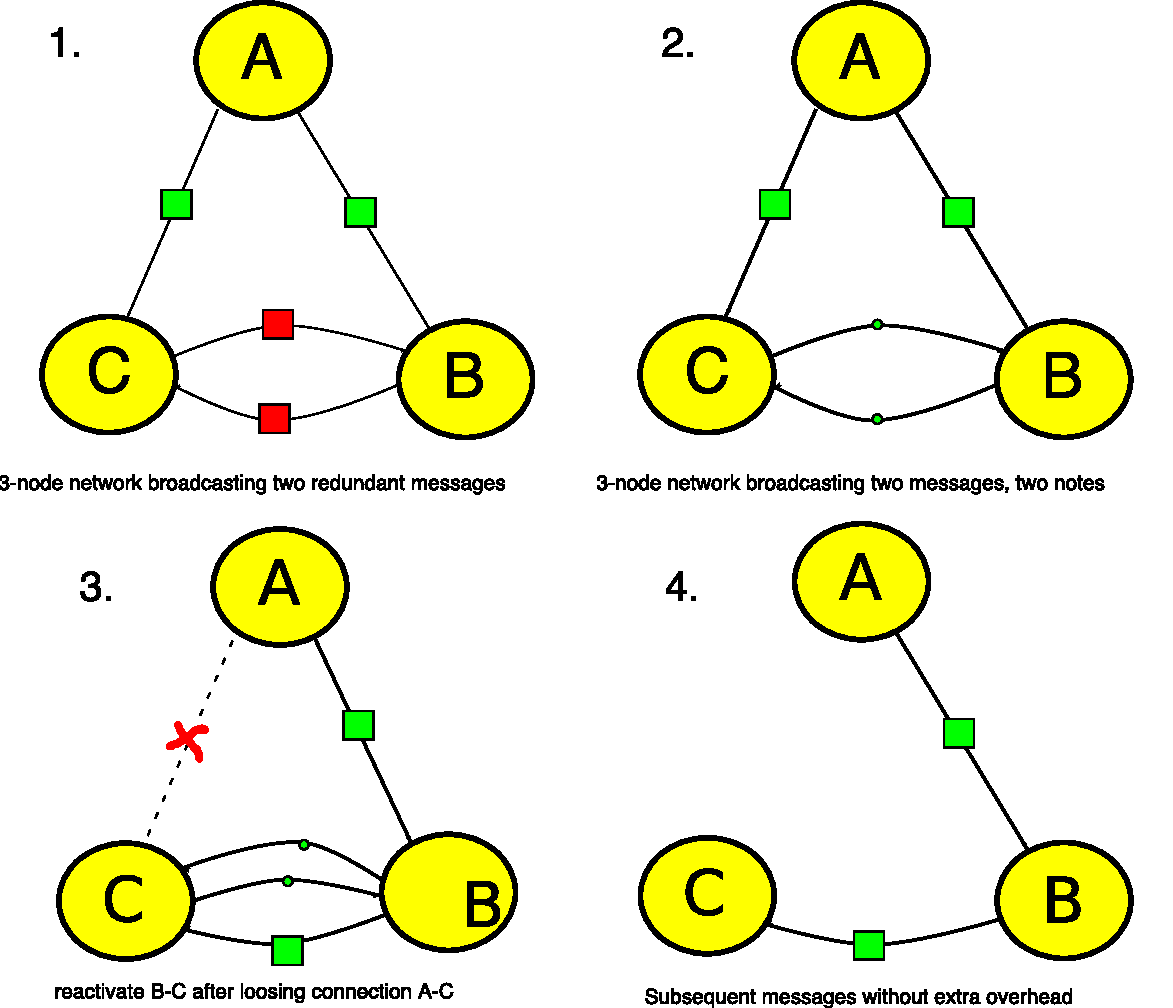
\includegraphics[width=0.9\columnwidth]{figs/redundant.pdf}

EBT still sends redundant data, but the notes sent along the redundant
connections are significantly smaller than the messages. Also, if a
delay is introduced, it is not necessary to send a note for every
message, but just the latest message.  If several are received in
quick succession, only one note needs to be sent.  Also, if a random
factor, somewhat greater than round trip time is added, then 50\% of
the time the same note is received before it is sent.

For example, B and C receive the message from A at approximately the
same time, if B decides to wait one second, and C waits two seconds,
and the note from B to C arrives in 0.1 seconds, C knows that B
already knows about that message, and now does not need to send a note
back.

\subsection{singleton hub}

{\em (footnote: To make the strongest arguement for the performance of
  EBT + request-skipping, compare it to a fully centralized model.}

To this point, most social networks have been implemented along a star
shaped network. Essentially one peer that distributes all messages to
all peers. If this was designed around a replication protocol, a
client would use something like the append-only poll, except the
server would remember each client's vector clock at each timestamp,
all their subscriptions, and the client would only send the time they
last synced.  The server would then send all new messages on any of
their subscriptions.

On each connection, the client needs to send their last connection
time, and the server still has to send each message. If a client polls
at low rate, the client sends one header and receives many
messages. If the client polls at a high rate, maybe they make one
request per message. (Long-lived connections would also help here.)

They would request the sequence number representing their own read
feed, on each connection they'd request any messages that have occured
since the last connection, but the central server still has to send
the messages.

`O(poll\_frequency + messages)`

the central server of course, must pay for a lot of resources,

bandwidth:

`O(network\_clients * poll\_frequency + peers * messages)`
and connections:

`O(network\_peers * poll\_frequency)`

If a network is successful, `network\_clients` can easily get very very
large: millions or billions of clients.

\subsection{conclusion}

An idealized centralized network is presented as the best possible in
efficiency, yet it only beats our design by a constant factor. Between
EBT with a fixed number of peers and request-skipping, we can manage
the bandwidth performance, but the main difference is only in vector
clock elements, which are very small compared to messages.

In the current secure-scuttlebutt implementation, which uses base64
encoded strings to encode 256 bit public keys plus a base 10 integer,
vector clock elements are about 60 bytes, and the average message is
660 bytes (although maximum message is 8kb) so the average message is
11 times bigger than a single vector clock element.

I would expect, that for a typical peer, most messages would be
replicated after being offline for a while, so one vector clock
element brings in many messages. For messages replicated in real-time,
the extra bandwidth used is managed by limiting the number of
connections.

The performance of our design is close enough to the optimal
centralized system to realistically argue that it's viable at massive
scale. In practice, we believe that small difference will easily be
made up by all the other advantages by adopting a decentralized
system.  For example, the significant costs associated with running
such a system are now spread around the network participants
evenly. With a fully decentralized gossip protocol, peers can join in
any topology. If two peers are offline, but nearby each other, it is
possible for them to share data directly over bluetooth, wifi, or by
directly exchanging physical media. This means secure-scuttlebutt is
potentially able to service remote areas of the earth that have not
yet received modern infrastructure, as well as areas where that
infrastructure is disrupted by warfare or other disasters.

% ----------------------------------------------------------------------
\end{document}

% eof
